% Options for packages loaded elsewhere
\PassOptionsToPackage{unicode}{hyperref}
\PassOptionsToPackage{hyphens}{url}
\PassOptionsToPackage{dvipsnames,svgnames,x11names}{xcolor}
%
\documentclass[
]{agujournal2019}

\usepackage{amsmath,amssymb}
\usepackage{iftex}
\ifPDFTeX
  \usepackage[T1]{fontenc}
  \usepackage[utf8]{inputenc}
  \usepackage{textcomp} % provide euro and other symbols
\else % if luatex or xetex
  \usepackage{unicode-math}
  \defaultfontfeatures{Scale=MatchLowercase}
  \defaultfontfeatures[\rmfamily]{Ligatures=TeX,Scale=1}
\fi
\usepackage{lmodern}
\ifPDFTeX\else  
    % xetex/luatex font selection
\fi
% Use upquote if available, for straight quotes in verbatim environments
\IfFileExists{upquote.sty}{\usepackage{upquote}}{}
\IfFileExists{microtype.sty}{% use microtype if available
  \usepackage[]{microtype}
  \UseMicrotypeSet[protrusion]{basicmath} % disable protrusion for tt fonts
}{}
\makeatletter
\@ifundefined{KOMAClassName}{% if non-KOMA class
  \IfFileExists{parskip.sty}{%
    \usepackage{parskip}
  }{% else
    \setlength{\parindent}{0pt}
    \setlength{\parskip}{6pt plus 2pt minus 1pt}}
}{% if KOMA class
  \KOMAoptions{parskip=half}}
\makeatother
\usepackage{xcolor}
\setlength{\emergencystretch}{3em} % prevent overfull lines
\setcounter{secnumdepth}{5}
% Make \paragraph and \subparagraph free-standing
\ifx\paragraph\undefined\else
  \let\oldparagraph\paragraph
  \renewcommand{\paragraph}[1]{\oldparagraph{#1}\mbox{}}
\fi
\ifx\subparagraph\undefined\else
  \let\oldsubparagraph\subparagraph
  \renewcommand{\subparagraph}[1]{\oldsubparagraph{#1}\mbox{}}
\fi


\providecommand{\tightlist}{%
  \setlength{\itemsep}{0pt}\setlength{\parskip}{0pt}}\usepackage{longtable,booktabs,array}
\usepackage{calc} % for calculating minipage widths
% Correct order of tables after \paragraph or \subparagraph
\usepackage{etoolbox}
\makeatletter
\patchcmd\longtable{\par}{\if@noskipsec\mbox{}\fi\par}{}{}
\makeatother
% Allow footnotes in longtable head/foot
\IfFileExists{footnotehyper.sty}{\usepackage{footnotehyper}}{\usepackage{footnote}}
\makesavenoteenv{longtable}
\usepackage{graphicx}
\makeatletter
\def\maxwidth{\ifdim\Gin@nat@width>\linewidth\linewidth\else\Gin@nat@width\fi}
\def\maxheight{\ifdim\Gin@nat@height>\textheight\textheight\else\Gin@nat@height\fi}
\makeatother
% Scale images if necessary, so that they will not overflow the page
% margins by default, and it is still possible to overwrite the defaults
% using explicit options in \includegraphics[width, height, ...]{}
\setkeys{Gin}{width=\maxwidth,height=\maxheight,keepaspectratio}
% Set default figure placement to htbp
\makeatletter
\def\fps@figure{htbp}
\makeatother
% definitions for citeproc citations
\NewDocumentCommand\citeproctext{}{}
\NewDocumentCommand\citeproc{mm}{%
  \begingroup\def\citeproctext{#2}\cite{#1}\endgroup}
\makeatletter
 % allow citations to break across lines
 \let\@cite@ofmt\@firstofone
 % avoid brackets around text for \cite:
 \def\@biblabel#1{}
 \def\@cite#1#2{{#1\if@tempswa , #2\fi}}
\makeatother
\newlength{\cslhangindent}
\setlength{\cslhangindent}{1.5em}
\newlength{\csllabelwidth}
\setlength{\csllabelwidth}{3em}
\newenvironment{CSLReferences}[2] % #1 hanging-indent, #2 entry-spacing
 {\begin{list}{}{%
  \setlength{\itemindent}{0pt}
  \setlength{\leftmargin}{0pt}
  \setlength{\parsep}{0pt}
  % turn on hanging indent if param 1 is 1
  \ifodd #1
   \setlength{\leftmargin}{\cslhangindent}
   \setlength{\itemindent}{-1\cslhangindent}
  \fi
  % set entry spacing
  \setlength{\itemsep}{#2\baselineskip}}}
 {\end{list}}
\usepackage{calc}
\newcommand{\CSLBlock}[1]{\hfill\break\parbox[t]{\linewidth}{\strut\ignorespaces#1\strut}}
\newcommand{\CSLLeftMargin}[1]{\parbox[t]{\csllabelwidth}{\strut#1\strut}}
\newcommand{\CSLRightInline}[1]{\parbox[t]{\linewidth - \csllabelwidth}{\strut#1\strut}}
\newcommand{\CSLIndent}[1]{\hspace{\cslhangindent}#1}

\usepackage{url} %this package should fix any errors with URLs in refs.
\usepackage{lineno}
\usepackage[inline]{trackchanges} %for better track changes. finalnew option will compile document with changes incorporated.
\usepackage{soul}
\linenumbers
\makeatletter
\@ifpackageloaded{caption}{}{\usepackage{caption}}
\AtBeginDocument{%
\ifdefined\contentsname
  \renewcommand*\contentsname{Table of contents}
\else
  \newcommand\contentsname{Table of contents}
\fi
\ifdefined\listfigurename
  \renewcommand*\listfigurename{List of Figures}
\else
  \newcommand\listfigurename{List of Figures}
\fi
\ifdefined\listtablename
  \renewcommand*\listtablename{List of Tables}
\else
  \newcommand\listtablename{List of Tables}
\fi
\ifdefined\figurename
  \renewcommand*\figurename{Figure}
\else
  \newcommand\figurename{Figure}
\fi
\ifdefined\tablename
  \renewcommand*\tablename{Table}
\else
  \newcommand\tablename{Table}
\fi
}
\@ifpackageloaded{float}{}{\usepackage{float}}
\floatstyle{ruled}
\@ifundefined{c@chapter}{\newfloat{codelisting}{h}{lop}}{\newfloat{codelisting}{h}{lop}[chapter]}
\floatname{codelisting}{Listing}
\newcommand*\listoflistings{\listof{codelisting}{List of Listings}}
\makeatother
\makeatletter
\makeatother
\makeatletter
\@ifpackageloaded{caption}{}{\usepackage{caption}}
\@ifpackageloaded{subcaption}{}{\usepackage{subcaption}}
\makeatother
\ifLuaTeX
  \usepackage{selnolig}  % disable illegal ligatures
\fi
\usepackage{bookmark}

\IfFileExists{xurl.sty}{\usepackage{xurl}}{} % add URL line breaks if available
\urlstyle{same} % disable monospaced font for URLs
\hypersetup{
  pdftitle={Near Infra-Red Spectroscopy Predicts Crude Protein in Hemp Grain},
  pdfauthor={Ryan Crawford; Jamie Crawford; Lawrence B. Smart; Virginia Moore},
  pdfkeywords={Hemp, Grain, Spectroscopy},
  colorlinks=true,
  linkcolor={blue},
  filecolor={Maroon},
  citecolor={Blue},
  urlcolor={Blue},
  pdfcreator={LaTeX via pandoc}}

\journalname{Earth and Space Science}

\draftfalse

\begin{document}
\title{Near Infra-Red Spectroscopy Predicts Crude Protein in Hemp Grain}

\authors{Ryan Crawford\affil{1}, Jamie Crawford\affil{1}, Lawrence B.
Smart\affil{2}, Virginia Moore\affil{3}}
\affiliation{1}{Cornell University, Ithaca, NY, }\affiliation{2}{Cornell
AgriTech, Geneva, NY, }\affiliation{3}{Cornell University, Ithaca, NY, }
\correspondingauthor{Ryan Crawford}{rvc3@cornell.edu}


\begin{abstract}
Lorem ipsum dolor sit amet, consectetur adipiscing elit, sed do eiusmod
tempor incididunt ut labore et dolore magna aliqua. Ut enim ad minim
veniam, quis nostrud exercitation ullamco laboris nisi ut aliquip ex ea
commodo consequat. Duis aute irure dolor in reprehenderit in voluptate
velit esse cillum dolore eu fugiat nulla pariatur. Excepteur sint
occaecat cupidatat non proident, sunt in culpa qui officia deserunt
mollit anim id est laborum.
\end{abstract}

\section*{Plain Language Summary}
Earthquake data for the island of La Palma from the September 2021
eruption is found \ldots{}



\textbf{incomplete: may contain errors, run-ons, half-thoughts, etc.}

\subsection{INTRODUCTION}\label{introduction}

Hemp (Cannabis sativa L.) is an annual crop with potential uses as a
source of food or feed from grain, and bast fiber or hurd from the
stalk. Hemp cultivars are commonly grown for one or both purposes and a
cultivar may be referred to as a grain, fiber, or dual-purpose type.
Because of protein's nutritional importance, the protein content of a
grain crop is an prime consideration for researchers, producers, and
consumers. Whole hemp grain typically contains approximately 25-30\%
protein (Bárta et al., 2024; Ely \& Fike, 2022). Crude protein (CP) is
often used as a proxy for the direct measurement of protein
concentration and consists of the multiplication of nitrogen
concentration by a conversion factor because measuring nitrogen
concentration is relatively easy and cheap via laboratory assay (Hayes,
2020).

Near-infrared spectroscopy (NIRS) technology is rapid, non-destructive,
and cheap, and consists of the measurement of NIR radiation reflected
from a sample (Roberts et al., 2004). NIR spectra from many samples are
related to laboratory values for components such as moisture, protein,
fat, or fiber {[}Roberts et al. (2004){]}. NIRS technology has been used
since the 1970's to assess forage CP (Reeves, 2012; Williams, 1975). A
NIRS calibration set often consists of samples from one species grown in
many environments encompassing the range of expected values from the
analyte or analytes (Chadalavada et al., 2022). Partial least squares
regression (PLSR) is a typical method used in the agricultural and food
sciences to relate spectra to analyte (Roberts et al., 2004).

A NIRS-scanned sample of undamaged grain may subsequently be grown, an
important consideration for a plant breeder. In wheat and corn, grain
protein content has been shown to be heritable {[}Giancaspro et al.
(2019); Geyer et al. (2022){]}. This suggests (at least potentially)
that NIRS technology could serve as resource to more rapidly identify
high CP hemp germplasm, senabling the delivery of higher CP hemp grain
cultivars faster.

For this study, a benchtop NIR spectrometer was used to develop a model
to predict CP content based on a data set representing multiple years,
locations, and cultivars using PLSR.

\subsection{MATERIALS AND METHODS}\label{materials-and-methods}

\textsubscript{Source:
\href{https://rvcrawford.github.io/glowing-system/index.qmd.html}{Article
Notebook}}

\subsubsection{Hemp Grain Sample
Background}\label{hemp-grain-sample-background}

Spectral data were obtained from whole (unground) hemp grain samples,
harvested at maturity, collected from 2017 - 2021 from 18 cultivar
trials in New York (NY) (149 samples). Grain samples were obtained by
hand sampling or mechanical harvest and were cleaned of chaff and dried
at 30 C for six days in a forced-air dryer. In total, 38 cultivars were
represented in the data set. Cultivars were grain or dual-purpose types
and included both commercially available and experimental material.

All cultivar trials were planted in randomized complete block design
with each cultivar replicated four times. The 2017 data were comprised
of samples from the same thirteen cultivars sampled from six NY
locations. For those trials, grain was harvested from each plot
individually and aggregated by cultivar within each trial. Four
subsamples were drawn from each aggregated sample and scanned
separately. These spectra were averaged at each 2 nm increment. All
remaining samples from 2018-2021 were collected on a per-plot basis. All
possible cultivars and possible locations were represented in 2017, but
only a selected subset of cultivars and locations were represented in
2018-2021.

\subsubsection{Spectral Data Collection and
Preprocessing}\label{spectral-data-collection-and-preprocessing}

A benchtop NIR spectrometer (FOSS/ NIR FOSS/ NIR Systems model 5000) was
used to obtain the spectra (FOSS North America, Eden Prairie, MN, USA).
Spectra were collected every 2 nm from 1100-2498 nm and the logarithm of
reciprocal reflectance was recorded.

WINISI software version 1.02A (Infrasoft International, Port Matilda,
PA, USA) was used to average the spectra in 2017, as well as to select
samples for laboratory assay. Samples were selected according to their
spectral distance from their nearest neighbor within the calibration
data set with a cutoff of a distance of 0.6 H, where H is approximately
equal to the squared Mahalanobis distance divided by the number of
principal components used in the calculation (Garrido-Varo et al.,
2019). Prior to selection selection, spectra were preprocessed using
SNV-detrend with settings 1,4,4,1 for the derivative, gap, smooth, and
smooth 2 settings respectively.

\subsubsection{Additional software
used:}\label{additional-software-used}

We used R version 4.3.3 (R Core Team, 2024) and the following R
packages: data.table v. 1.15.2 (Barrett et al., 2024), randomForest v.
4.7.1.1 (Liaw \& Wiener, 2002), rmarkdown v. 2.26 (Allaire et al., 2024;
Xie et al., 2018, 2020), tidyverse v. 2.0.0 (Wickham et al., 2019).

\textsubscript{Source:
\href{https://rvcrawford.github.io/glowing-system/index.qmd.html}{Article
Notebook}}

\subsubsection{Preprocessing}\label{preprocessing}

Multiplicative scatter correction (MSC)

standard normal variate (SNV) transformation

The calibration set consisted of

The validation set consisted of

\subsubsection{Laboratory Validation}\label{laboratory-validation}

Laboratory assays were performed by Dairy One Forage Laboratory (Ithaca,
NY). For those assays, 1mm ground samples were analyzed by combustion
using a CN628 or CN928 Carbon/Nitrogen Determinator. Samples from 2017
were aggregated as described above, but

Prior to In 2017, an in

\subsection{RESULTS AND DISCUSSION}\label{results-and-discussion}

\subsection{ACKNOWLEDGMENTS}\label{acknowledgments}

\subsection{SUPPLEMENTAL MATERIAL}\label{supplemental-material}

\subsection{OPTIONAL SECTIONS}\label{optional-sections}

\subsection{REFERENCES}\label{references}

\subsection{FIGURES AND TABLES}\label{figures-and-tables}

\textsubscript{Source:
\href{https://rvcrawford.github.io/glowing-system/index.qmd.html}{Article
Notebook}}

\phantomsection\label{cell-fig-timeline}
\begin{figure}[H]

\centering{

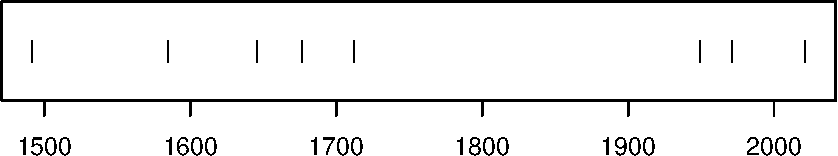
\includegraphics{index_files/figure-pdf/fig-timeline-1.pdf}

}

\caption{\label{fig-timeline}Timeline of recent earthquakes on La Palma}

\end{figure}%

\textsubscript{Source:
\href{https://rvcrawford.github.io/glowing-system/index.qmd.html}{Article
Notebook}}

\textsubscript{Source:
\href{https://rvcrawford.github.io/glowing-system/index.qmd.html}{Article
Notebook}}

Based on data up to and including 1971, eruptions on La Palma happen
every 79.8 years on average.

Studies of the magma systems feeding the volcano, such as
(\textbf{marrero2019?}), have proposed that there are two main magma
reservoirs feeding the Cumbre Vieja volcano; one in the mantle (30-40km
depth) which charges and in turn feeds a shallower crustal reservoir
(10-20km depth).

Eight eruptions have been recorded since the late 1400s
(Figure~\ref{fig-timeline}).

Data and methods are discussed in Section~\ref{sec-data-methods}.

Let \(x\) denote the number of eruptions in a year. Then, \(x\) can be
modeled by a Poisson distribution

\begin{equation}\phantomsection\label{eq-poisson}{
p(x) = \frac{e^{-\lambda} \lambda^{x}}{x !}
}\end{equation}

where \(\lambda\) is the rate of eruptions per year. Using
Equation~\ref{eq-poisson}, the probability of an eruption in the next
\(t\) years can be calculated.

\begin{longtable}[]{@{}ll@{}}
\caption{Recent historic eruptions on La
Palma}\label{tbl-history}\tabularnewline
\toprule\noalign{}
Name & Year \\
\midrule\noalign{}
\endfirsthead
\toprule\noalign{}
Name & Year \\
\midrule\noalign{}
\endhead
\bottomrule\noalign{}
\endlastfoot
Current & 2021 \\
Teneguía & 1971 \\
Nambroque & 1949 \\
El Charco & 1712 \\
Volcán San Antonio & 1677 \\
Volcán San Martin & 1646 \\
Tajuya near El Paso & 1585 \\
Montaña Quemada & 1492 \\
\end{longtable}

Table~\ref{tbl-history} summarises the eruptions recorded since the
colonization of the islands by Europeans in the late 1400s.

\begin{figure}

\centering{

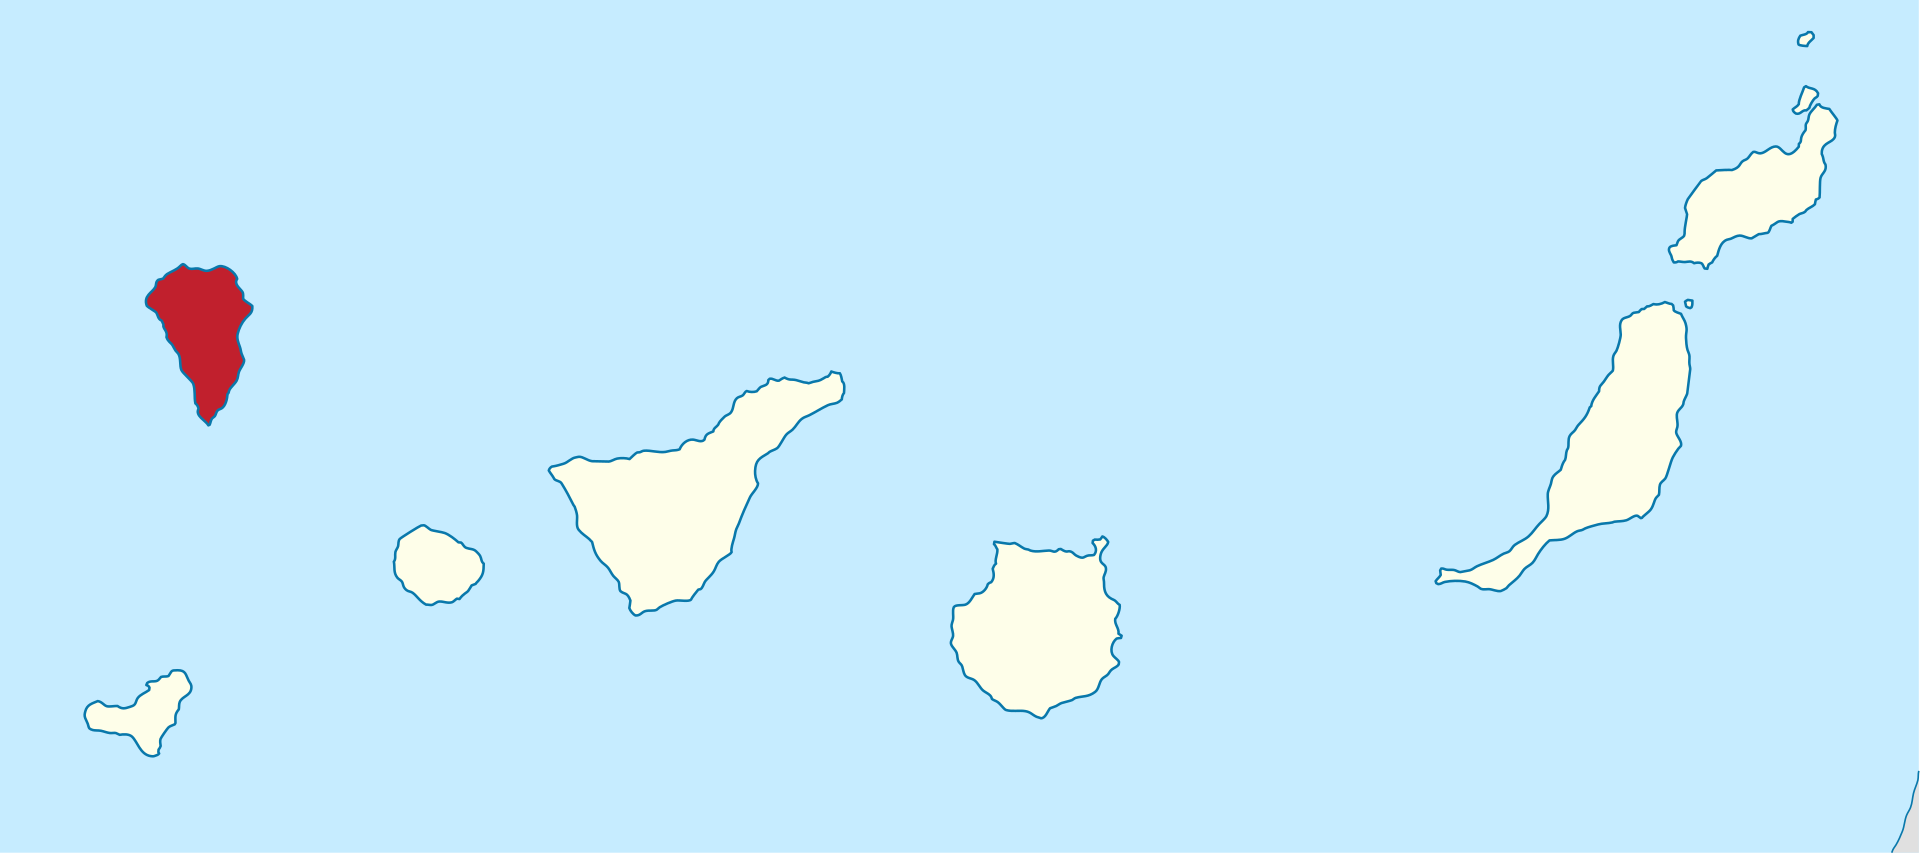
\includegraphics{images/la-palma-map.png}

}

\caption{\label{fig-map}Map of La Palma}

\end{figure}%

La Palma is one of the west most islands in the Volcanic Archipelago of
the Canary Islands (Figure~\ref{fig-map}).

\begin{figure}[H]

\centering{

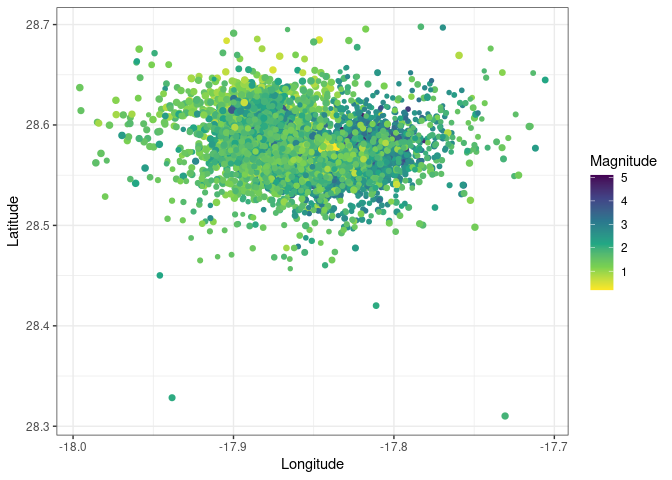
\includegraphics{index_files/figure-latex/notebooks-explore-earthquakes-fig-spatial-plot-output-1.png}

}

\caption{\label{fig-spatial-plot}Locations of earthquakes on La Palma
since 2017}

\end{figure}%

\textsubscript{Source:
\href{https://rvcrawford.github.io/glowing-system/notebooks/explore-earthquakes-preview.html\#cell-fig-spatial-plot}{Explore
Earthquakes}}

Figure~\ref{fig-spatial-plot} shows the location of recent Earthquakes
on La Palma.

\subsection{Data \& Methods}\label{sec-data-methods}

\subsection{Conclusion}\label{conclusion}

\subsection*{References}\label{references-1}
\addcontentsline{toc}{subsection}{References}

\phantomsection\label{refs}
\begin{CSLReferences}{1}{0}
\vspace{1em}

\bibitem[\citeproctext]{ref-rmarkdown2024}
Allaire, J., Xie, Y., Dervieux, C., McPherson, J., Luraschi, J., Ushey,
K., Atkins, A., Wickham, H., Cheng, J., Chang, W., \& Iannone, R.
(2024). \emph{{rmarkdown}: Dynamic documents for r}.
\url{https://github.com/rstudio/rmarkdown}

\bibitem[\citeproctext]{ref-datatable}
Barrett, T., Dowle, M., Srinivasan, A., Gorecki, J., Chirico, M., \&
Hocking, T. (2024). \emph{{data.table}: Extension of
{``{data.frame}''}}. \url{https://CRAN.R-project.org/package=data.table}

\bibitem[\citeproctext]{ref-barta_proteomic_2024}
Bárta, J., Roudnický, P., Jarošová, M., Zdráhal, Z., Stupková, A.,
Bártová, V., Krejčová, Z., Kyselka, J., Filip, V., Říha, V., Lorenc, F.,
Bedrníček, J., \& Smetana, P. (2024). Proteomic {Profiles} of {Whole}
{Seeds}, {Hulls}, and {Dehulled} {Seeds} of {Two} {Industrial} {Hemp}
({Cannabis} sativa {L}.) {Cultivars}. \emph{Plants}, \emph{13}(1), 111.
\url{https://doi.org/10.3390/plants13010111}

\bibitem[\citeproctext]{ref-chadalavada_nir_2022}
Chadalavada, K., Anbazhagan, K., Ndour, A., Choudhary, S., Palmer, W.,
Flynn, J. R., Mallayee, S., Pothu, S., Prasad, K. V. S. V.,
Varijakshapanikar, P., Jones, C. S., \& Kholová, J. (2022). {NIR}
{Instruments} and {Prediction} {Methods} for {Rapid} {Access} to {Grain}
{Protein} {Content} in {Multiple} {Cereals}. \emph{Sensors (Basel,
Switzerland)}, \emph{22}(10). \url{https://doi.org/10.3390/s22103710}

\bibitem[\citeproctext]{ref-ely_industrial_2022}
Ely, K., \& Fike, J. (2022). Industrial {Hemp} and {Hemp} {Byproducts}
as {Sustainable} {Feedstuffs} in {Livestock} {Diets}. In D. C. Agrawal,
R. Kumar, \& M. Dhanasekaran (Eds.), \emph{Cannabis/{Hemp} for
{Sustainable} {Agriculture} and {Materials}} (pp. 145--162). Springer.
\url{https://doi.org/10.1007/978-981-16-8778-5_6}

\bibitem[\citeproctext]{ref-garrido-varo_note_2019}
Garrido-Varo, A., Garcia-Olmo, J., \& Fearn, T. (2019). A note on
{Mahalanobis} and related distance measures in {WinISI} and {The}
{Unscrambler}. \emph{Journal of Near Infrared Spectroscopy},
\emph{27}(4), 253--258. \url{https://doi.org/10.1177/0967033519848296}

\bibitem[\citeproctext]{ref-geyer_genetics_2022}
Geyer, M., Mohler, V., \& Hartl, L. (2022). Genetics of the {Inverse}
{Relationship} between {Grain} {Yield} and {Grain} {Protein} {Content}
in {Common} {Wheat}. \emph{Plants}, \emph{11}(16), 2146.
\url{https://doi.org/10.3390/plants11162146}

\bibitem[\citeproctext]{ref-giancaspro_genetic_2019}
Giancaspro, A., Giove, S. L., Blanco, A., \& Gadaleta, A. (2019).
Genetic {Variation} for {Protein} {Content} and {Yield}-{Related}
{Traits} in a {Durum} {Population} {Derived} {From} an
{Inter}-{Specific} {Cross} {Between} {Hexaploid} and {Tetraploid}
{Wheat} {Cultivars}. \emph{Frontiers in Plant Science}, \emph{10}.
\url{https://doi.org/10.3389/fpls.2019.01509}

\bibitem[\citeproctext]{ref-hayes_measuring_2020}
Hayes, M. (2020). Measuring {Protein} {Content} in {Food}: {An}
{Overview} of {Methods}. \emph{Foods}, \emph{9}(10), 1340.
\url{https://doi.org/10.3390/foods9101340}

\bibitem[\citeproctext]{ref-randomForest}
Liaw, A., \& Wiener, M. (2002). Classification and regression by
randomForest. \emph{R News}, \emph{2}(3), 18--22.
\url{https://CRAN.R-project.org/doc/Rnews/}

\bibitem[\citeproctext]{ref-base}
R Core Team. (2024). \emph{{R}: A language and environment for
statistical computing}. R Foundation for Statistical Computing.
\url{https://www.R-project.org/}

\bibitem[\citeproctext]{ref-reeves_potential_2012}
Reeves, J. B. (2012). Potential of {Near}- and {Mid}-infrared
{Spectroscopy} in {Biofuel} {Production}. \emph{Communications in Soil
Science and Plant Analysis}, \emph{43}(1-2), 478--495.
\url{https://doi.org/10.1080/00103624.2012.641844}

\bibitem[\citeproctext]{ref-roberts_near-infrared_2004}
Roberts, C. A., Workman, J., \& Reeves, J. B. (2004).
\emph{Near-infrared spectroscopy in agriculture}. American Society of
Agronomy.

\bibitem[\citeproctext]{ref-tidyverse}
Wickham, H., Averick, M., Bryan, J., Chang, W., McGowan, L. D.,
François, R., Grolemund, G., Hayes, A., Henry, L., Hester, J., Kuhn, M.,
Pedersen, T. L., Miller, E., Bache, S. M., Müller, K., Ooms, J.,
Robinson, D., Seidel, D. P., Spinu, V., \ldots{} Yutani, H. (2019).
Welcome to the {tidyverse}. \emph{Journal of Open Source Software},
\emph{4}(43), 1686. \url{https://doi.org/10.21105/joss.01686}

\bibitem[\citeproctext]{ref-williams_application_1975}
Williams, P. C. (1975). Application of near infrared reflectance
spectroscopy to analysis of cereal grains and oilseeds. \emph{Cereal
Chemistry}, \emph{52}(4 p.561-576), 576--561.

\bibitem[\citeproctext]{ref-rmarkdown2018}
Xie, Y., Allaire, J. J., \& Grolemund, G. (2018). \emph{R markdown: The
definitive guide}. Chapman; Hall/CRC.
\url{https://bookdown.org/yihui/rmarkdown}

\bibitem[\citeproctext]{ref-rmarkdown2020}
Xie, Y., Dervieux, C., \& Riederer, E. (2020). \emph{R markdown
cookbook}. Chapman; Hall/CRC.
\url{https://bookdown.org/yihui/rmarkdown-cookbook}

\end{CSLReferences}



\end{document}
